\documentclass{llncs}
\usepackage{makeidx}  % allows for indexgeneration
\usepackage{graphicx}
\usepackage{subfig}
\usepackage{float}
\graphicspath{{images/}}
\begin{document}
\frontmatter          % for the preliminaries
\pagestyle{headings}  % switches on printing of running heads
\mainmatter              % start of the contributions


\title{Semantic Segmentation of Cilia using Fully-Convolutional Dense Networks}
\titlerunning{Cilia Segmentation}  % abbreviated title (for running head)
\author{Charles Lu \and
Shannon Quinn}
\authorrunning{Charles Lu} % abbreviated author list (for running head)
%%%% list of authors for the TOC (use if author list has to be modified)
\tocauthor{}
\institute{University of Georgia, Athens GA 30605, USA,\\
\email{\{clu, squinn\}@cs.uga.edu}}
\maketitle              % typeset the title of the contribution


\begin{abstract}
Cilia are hairlike structures protruding from nearly every cell in the body. Diseases known as ciliopathies with disruption of nonmotile or motile cilia function can result in a wide spectrum of diseases. However, most techniques for assessing ciliary motion rely on manual identification and tracking of cilia. This annotation is tedious and error-prone, whereas more analytical techniques impose strong assumptions such as periodic motion of beating cilia. Deep convolutional networks are able to encode complex features while remaining sensitive enough to segment cilia that exhibit a variety of motion patterns. We compare fully convolutional networks with dense connections to a baseline model without dense connections for the novel task of automated cilia segmentation from frames of biopsy videos. Trained on only 235 labeled images, our fully convolutional DenseNet achieves an overall pixel accuracy of 90.15\%, which is 14\% more accurate than U-Net with 10x fewer parameters. We demonstrate the utility and parameter efficiency of DenseNets for semantic segmentation of small biomedical datasets, and anticipate this method could be used in a larger automated ciliary motion analysis pipeline.

 \keywords{Cilia, Ciliopathies, Semantic Segmentation, DenseNets, Fully Convolutional DenseNets}
\end{abstract}


\section{Introduction}

Cilia help to regulate the respiratory system by generating fluid flow to deliver nutrients and propel out mucus and foreign matter. These hairlike structures on the cell body are vital in reproduction, homeostasis, and  organs development. Defects in ciliary motion have been associated with a wide range of diseases such as birth defects, sinopulmonary infection, and congenital heart disease \cite{Ciliopathy}. Assessment of ciliary motion from biopsy videos relies on accurate detection and segmentation of cilia from the surrounding cell, a task that even in a recent ciliary motion analysis pipelines remains as manual labor~\cite{QuinnSTM}. Therefore, accurate and fully automated segmentation of motile cilia provides clinical significance in the identification and further study of ciliopathies and their underlying motion patterns. 
\par 
Current methods of ciliopathy identification and diagnosis rely on an ensemble of techniques. Electron microscopy (EM) can elucidate structural defects that connect to certain ciliopathies, but some ciliopathies present without any discernible structural deformities~\cite{CiliaEM}. Examining ciliary beat pattern from videos of ciliary biopsies is among the most promising methods, but this is usually conducted manually; consequently it is tedious and time-consuming, and the eventual conclusions are highly subjective~\cite{CiliaCM}. Furthermore, there is little consensus on deterministic definitions of ciliary motion phenotypes, ruling out any possibility of cross-institutional collaboration. While \cite{QuinnSTM} proposed a promising initial ciliary motion quantification pipeline, it was limited in its reliance on manually-selected regions of interest on which to operate. Therefore, a fast and reliable method automating the region-of-interest selection process is desirable to clinicians and researchers, accelerating the adoption of objective ciliary motion measures and bringing an end-to-end ciliary motion analysis pipeline closer to fruition. To our knowledge, no computational pipeline for semantic cilia segmentation from microscopy images has been proposed using deep learning techniques. 
\par
Deep learning approaches to semantic segmentation have gained state of the art performance on many benchmark datasets in biomedical imaging. The task of cilia segmentation is challenging due to their size, shape, and orientation. A single cilium can present itself in only a few pixels in an image depending on its orientation to the camera perspective. In addition, the hairlike shape of cilia can easily be mistaken for extraneous recording artifacts such as poor focus, inconsistent lighting, and blur from a shaky camera perspective.
\par
Another challenge in cilia detection is the assumption and reliance of temporal information about cilia. A model for automatic detection of cilia should ideally be able to segment and classify cilia that do not display a regular motion; diseased ciliary motion patterns may show little, if any, motility, thus the segmentation model should be able to identify cilia from a single frame of microscopy video.
\par 
Fully convolutional networks (FCN) \cite{FCN} comprise of a feature extractor that feeds into an upsampling path to recover back an image of the predicted segmentation mask. Shortcut or skip connections can be introduced between the downsampling and upsampling paths to allow for passing of feature information to deeper layers \cite{Highway}. These skip connection allow for deep networks to be trained as the gradient can flow propagate more easily from deep layers. This type of architecture has been applied to biomedical imaging data as an end-to-end model for segmentation tasks \cite{U-Net}.
\par
DenseNets \cite{DenseNet} extend the idea of shortcut connections by concatenating the feature maps of each layer to every other layer in the same dense block, similar to Inception style networks \cite{Inception}, effectively maximizing the information flow between layers. While densely connected layers add more parameters per layer due to increased number of shortcut connections, the overall number of parameters is reduced because less feature maps are needed in each layer. This property allows DenseNets to be very deep while remaining extremely parameter efficient. We propose that this attribute also makes DenseNets excellent for small datasets because dense connections naturally reduce overfitting and eliminate the need for heavy regularization in some cases.    
\par
Our main contributions in this paper are as follows:
\begin{itemize}
\item establish an accurate and reliable computational model for semantic segmentation of cilia from a single frame of microscopy video,
\item compare the performance of fully convolutional networks with dense connections to a baseline FCN without dense connections on the novel task of cilia segmentation, and 
\item highlight the advantageous properties of DenseNets that make this architecture extremely suitable for biomedical data with few labeled examples.  
\end{itemize}


\section{Methods}

In DenseNets, each layer has direct access to the gradients from loss and original input. The number of feature maps in each layer is controlled by a growth parameter $k$ We implement a version of the Tiramisu network \cite{Tiramisu} with a growth rate $k = 16$ and train several models with different depths and hyper-parameter settings. 

\subsection{Network Architecture}
The Network comprises of dense blocks in both the downsampling and upsampling paths. Dense blocks are followed by transition down blocks in the downsampling path and preceded by transition up block in the upsampling path. More layers are stacked in each dense block until the bottleneck dense block in the middle of the network after which the number of layers decease in each subsequent dense block. Ship connections connect dense blocks in the downsampling and upsampling paths, facilitating information flow from earlier layers so that high-level features can be reused in deeper layers. A convolutional layer is added before the first block and after the last block. An overview of the architecture for a fully convolutional DenseNet with 74 layers is shown in figure 1.

\begin{figure}
\centering
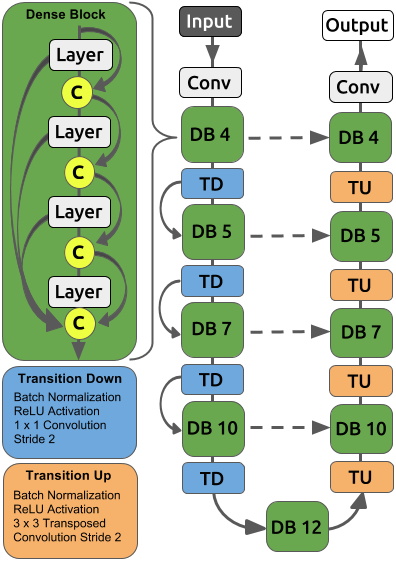
\includegraphics[width=8cm, height=10cm]{densenet}
\caption{Diagram of FC-DenseNet 74. Yellow circles represent the concatenation operation and dashed lines represent skip connections.}
\end{figure}

\subsection{Dense Blocks}
Whereas in Residual blocks \cite{ResNet} sum an identity mapping with a nonlinear transformation, dense blocks (DB) use the concatenation operation to maximize feature reuse between all layers in a DB to ease the flow of gradients to earlier layers during backpropagation. Layers in a DB are iteratively concatenated with the number of connections with layer $L$ having  $\frac{L\left(2+1\right)}{2}$ connections instead of just $L$. This means the number of feature maps in a DenseNet increase linearly with depth. Each layer in a DB comprises of a Batch Normalization \cite{Batchnorm} followed by a $3 \times 3$ convolution with Rectified Linear Units \cite{ReLU}. Dropout \cite{Dropout} and weight decay regularization are added to control overfitting.  

\subsection{Transition Blocks}
Transition down (TD) blocks reduce dimensionality of the feature maps. To this end, TD blocks contain a $ 1 \times 1$ convolution with Batch Normalization, ReLU activations, and Dropout. In the original Tiramisu paper \cite{Tiramisu}, $2 \times 2$ max pooling is used in the TD blocks, however we find that using a stride of 2 instead obtains better results. In FC-DenseNet, Transition up (TU) and dense blocks replace the upsampling path of a FCN. TU blocks consist of $3 \times 3$ transposed convolutions with stride 2 to match the stride of the downsampling path.   

\subsection{Training}
We train FC-DenseNets with different number of layers to study the optimal tradeoff between speed and accuracy. The Adam \cite{Adam} optimizer was used to minimize the loss function and we vary several regularization parameters tunings: dropout, $l^2$ weight decay, and learning rate annealing. All models weights were initialized with HeUniform initialization \cite {ReLU}. Each model was trained for 100 epochs with a batch size of 4 on $2  \times$ Titan X GPU and all models were implemented in Tensorflow with Keras \cite{TensorFlow,Keras}.


\section{Experiment}

\subsection{Data}
325 grayscale videos from two separate video cohorts of nasal brush biopsies were collected from 149 patients (data from ~\cite{QuinnSTM}; see it for details on patient recruitment, nasal biopsy extraction, and spectroscopic techniques and technologies). Each video depicted cilia along with varying levels of recording artifacts such as extraneous camera movement, uneven lighting, or poor focus. A cilium structure observed vertically to the camera's perspective appears very different than a cilium lining the side of the cell body. To address this, we separate cilia annotations into \textit{side} cilia and \textit{top} cilia class labels. Four class annotations (side, cilia, top cilia, cell body, and background) were manually segmented out using ITK-SNAP \cite{ITK-SNAP}.
\par
Only the first frame of each video is used so that the model avoids relying on any information about ciliary motion in the temporal dimension for segmentation. The pixels were normalized by subtracting the mean pixel value and dividing by the standard deviation. The dimension of each image varied in resolution so all images were resized to $224 \times 224$ pixels and transformed by random flips to augment the data. We set aside 75 of the 325 images as a holdout test set and randomly choose samples from the remaining 250 for training and validation using a $60/40$\% train-validation split.

\subsection{Evaluation Metric}
Because the task is multi-class segmentation, we train the optimizer to minimize sparse categorical cross entropy to account for the skew in distribution of pixel class labels. We evaluate models on overall pixel classification accuracy, using the class with the highest probability for each pixel as the predicted pixel class. Categorical cross entropy is defined as:
\begin{equation}
L_{cce} = -\frac{1}{n}\sum^n_{i=1}\sum^c_{j=i}\ y_{ij}\ log\left(p_{ij}\right)
\end{equation}
where $i$ indexes samples, $j$ indexes the number of classes, $y$ is the sample label, and $p_{ij} \in (0, 1) \; s.t. \sum_j p_{ij} = 1$.

The dice coefficient loss is defined as:
\begin{equation}
L_{Dice} = -\frac{2 \sum_i p_{ij} y_{ij}}{\sum_i p_{ij} + \sum_i y_{ij}}
\end{equation}

\subsection{Baseline}
We select a U-Net \cite{U-Net} architecture model as our baseline as it incorporates skip connections between the downsampling and upsampling paths, similar to our DenseNet model. The baseline model uses pre-trained weights on ImageNet \cite{Imagenet}.   

\setlength{\tabcolsep}{3pt}
\begin{table}
	\centering
	\begin{tabular}{c | c | c | c | c | c | c}
		\hline
		Model & Parameters & Pre-trained & Dropout & Decay & Dice Loss & Accuracy \\ 
		\hline
		U-Net & 30 M & Yes & 0.3 & 0.001 & * & 76.90\% \\ 
		FC-DenseNet 50 & 1.7 M & No & 0.2 & 0.001 & * & 85.23\% \\ 
		FC-DenseNet 74 & 3.7 M & No & 0.1 & 0.0001 & * & 87.59\% \\ 
		FC-DenseNet 103 & 9.6 M & No & 0.1 & None & * & 89.27\% \\
		FC-DenseNet 136 & 33 M & No & None & None & * & 90.15\% \\
	\end{tabular}
	\bigskip
	\caption{Table of results. The parameters are represented in millions.}
\end{table}
\vspace{-4em}

\subsection{Results}
The best model attains, on average, 90.15\% overall pixel accuracy on the holdout test set. This is a about 13\% more accurate than the U-Net baseline. Even the FC-DenseNet with 50 layers is 8\% more accurate than the baseline. This difference in performance is considerable especially since FC-DenseNet 50 has $10 \times$ fewer parameters than the baseline. In addition, despite achieving better performance, none of the DenseNet models were pre-trained on ImageNet. DenseNets also needed less regularization and converged to a minima faster than the baseline model.

\begin{figure}[t]
\centering
\begin{tabular}{c c c c}
\subfloat{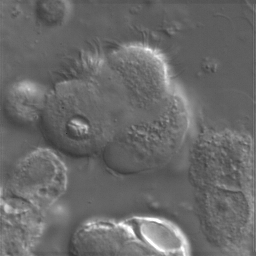
\includegraphics[width=3cm,height=3cm]{9013g.png}} &
\subfloat{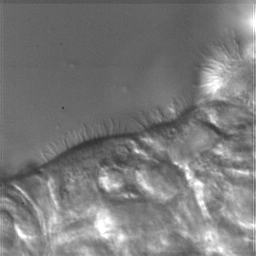
\includegraphics[width=3cm,height=3cm]{9028-1.png}} &
\subfloat{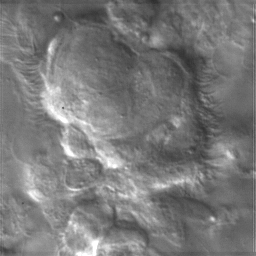
\includegraphics[width=3cm,height=3cm]{90232.png}} &
\subfloat{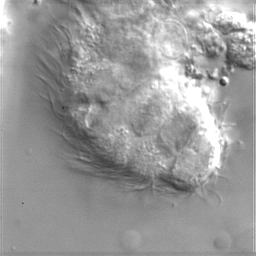
\includegraphics[width=3cm,height=3cm]{90254.png}} \\ [-2ex]

\subfloat{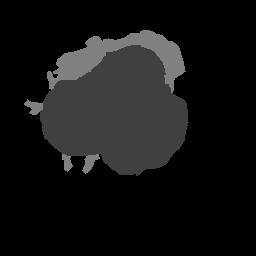
\includegraphics[width=3cm,height=3cm]{9013g_m.png}} &
\subfloat{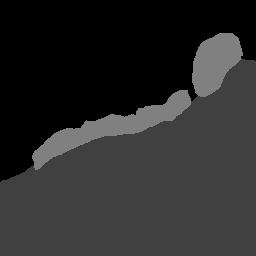
\includegraphics[width=3cm,height=3cm]{9028-1_m.png}} &
\subfloat{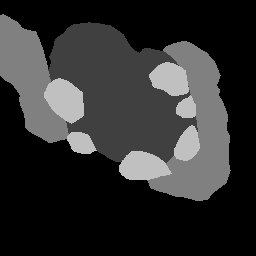
\includegraphics[width=3cm,height=3cm]{90232_m.png}} &
\subfloat{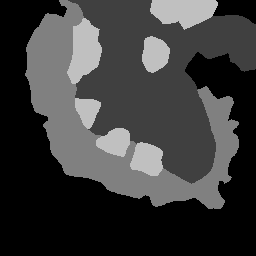
\includegraphics[width=3cm,height=3cm]{90254_m.png}} \\ [-2ex]

\subfloat{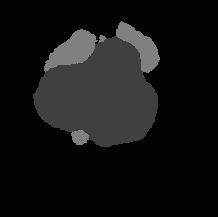
\includegraphics[width=3cm,height=3cm]{0.png}} &
\subfloat{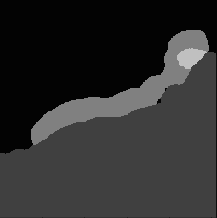
\includegraphics[width=3cm,height=3cm]{1.png}} &
\subfloat{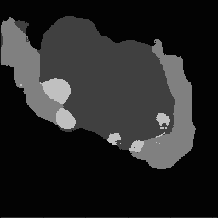
\includegraphics[width=3cm,height=3cm]{3.png}} &
\subfloat{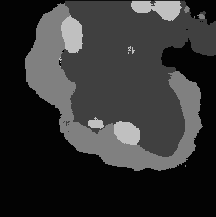
\includegraphics[width=3cm,height=3cm]{2.png}} \\ [-2ex]
\end{tabular}
\caption{Top row depicts grayscale frames of microscopy images. Middle row depicts ground truth masks. Bottom row is the predicted masks. Black represents the background class; dark gray represents the cell body; medium gray represents the side cilia, light gray represents the top cilia.}
\end{figure}

\subsection{Benefits of Dense Connections}
These results show that dense connections are extremely efficient in facilitating increased the flow of information and gradients between layers. This allows the network to reuse feature maps and act as natural regularization by making information from earlier layers available to later layers. 
\par
This is similar to  Implicit Deep Supervision from loss function by shorter connections but with the added benefit of being less complicated than DSN. \cite{Stochastic} show that each individual layer in ResNets \cite{ResNet} contribute little to the model overall and can be randomly dropped out during training. This redundancy in features is avoided in DenseNets through their dense connections, acting as a kind of inherent multi-scale supervision \cite{DSN}. Because there is no need to relearn redundant feature maps in a DenseNet, there is less need for regularization, and in our experiments we found that too much regularization to even degrade performance accuracy. 
 \par
Sometimes the FC-DenseNet correctly predicted background cilia even when they were not annotated in the ground truth. Additionally, there is some ambiguity in the distinction between side and top cilia in the manual annotations. After demonstrating the effectiveness of segmentation from a single frame, subsequent frames of the video could be taken into context to alleviate some of this ambiguity and further refine prediction by incorporating the temporal dimension. 
 \par
Unlike most fully convolutional networks, FC-DenseNets achieve excellent results without the need for pre-trained weights or post-processing steps such as Conditional Random Fields (CRF) to finetune the segmentation masks  \cite{DeepLab,CRF}. However, since our model is trainable end-to-end, using transfer learning \cite{Transfer} and pre-training or CRF post-processing might well boost model performance even more.  


\section{Conclusion}
In this paper, we demonstrate the efficacy of a fully convolutional DenseNet on the challenging task of cilia segmentation and explore the implicit regularizing properties inherent to this network architecture. We also highlight the advantageous properties of fully convolution DenseNets for biomedical datasets with few labels for semantic segmentation. We plan to incorporate the semantic segmentation model into our previous ciliary motion analysis pipeline to increase the overall automation, permitting analysis of vastly larger data cohorts as we ultimately seek to characterize and quantify discrete ciliary motion subtypes and understand their roles in certain ciliopathies.

\section*{Acknowledgements}
We would like to thank all the developers of Tensroflow and Keras for providing extremely powerful  frameworks for deep learning.  We  t? gratefully  acknowledge  NVIDIA  for  GPU  donation to  our  lab  at?Ecole  Polytechnique.  The  authors  would  like  to  thank  Lisa  diJorio,  Adriana  Romero  and  Nicolas  Chapados  for  insightful  discussions.  

\begin{thebibliography}{26}

\bibitem{CiliaCM}
Raidt, J. et al.:
Ciliary beat pattern and frequency in genetic variants of primary ciliary dyskinesia.
European Respiratory Journal, pp. erj00520--2014 (2014).

\bibitem{CiliaEM}
Stannard, W.A., Chilvers, M.A., Rutman, A.R., Williams, C.D., O'Callaghan, C.:
Diagnostic testing of patients suspected of primary ciliary dyskinesia.
American journal of respiratory and critical care medicine, 181(4), pp. 307--314 (2010)

\bibitem{QuinnSTM}
Quinn, S., Zahid, M.J., Durkin, J.R., Francis, R.J., Lo, C.W., Chennubhotla, S.C.:
Automated identification of abnormal respiratory ciliary motion in nasal biopsies.
Science Translational Medicine, 7(299), pp. 299ra124--299ra124 (2015)

\bibitem{TensorFlow}
Abadi, M., et al.:
TensorFlow: Large-Scale Machine Learning on Heterogeneous Distributed Systems.
CoRR abs/1603.04467 (2016)

\bibitem{DeepLab}
Chen, L., Papandreou, G., Kokkinos, I., Murphy, K., Yuille, A.:
DeepLab: Semantic Image Segmentation with Deep Convolutional Nets, Atrous Convolution, and Fully Connected CRFs.
CoRR abs/1606.00915 (2016)

\bibitem{Keras}
Chollet, F.:
Keras.
\url{https://github.com/fchollet/keras} (2015)

\bibitem{Imagenet}
Deng, J., Dong, W., Socher, R., Li, L.-J., Li, k., Fei-Fei, L.:
ImageNet: A Large-Scale Hierarchial Image Database.
Conference on Computer Vision and Pattern Recognition (2009)

\bibitem{Skip}
Drozdzal, M., Vorontsov, E., Chartrand, G., Kadoury, S., Pal, C.:
The Importance of Skip Connections in Biomedical Image Segmentation.
CoRR abs/1608.04117 (2016)

\bibitem{ResNet}
He, K., Zhang, X., Ren, S., Sun, J.:
Deep Residual Learning for Image Recognition.
CoRR abs/1512.03385 (2015)

\bibitem{ReLU}
He, K., Zhang, X., Ren, S., Sun, J.:
Delving Deep into Rectifiers: Surpassing Human-Level Performance on ImageNet Classification.
CoRR abs/1502.01852 (2015)

\bibitem{DenseNet}
Huang, G., Liu, Z., Weinberger, K.:
Densely Connected Convolutional Networks.
CoRR abs/1608.06993 (2016)

\bibitem{Stochastic}
Huang, G., Sun, Y., Liu, Z., Sedra, D., Weinberger, K.:
Deep Networks with Stochastic Depth.
CoRR abs/1603.09382 (2016)

\bibitem{Batchnorm}
Ioffe, S., Szegedy, C.:
Batch Normalization: Accelerating Deep Network Training by Reducing Internal Covariate Shift.
CoRR abs/1502.03167 (2015)

\bibitem {Tiramisu}
J{\'{e}}gou, S., Drozdzal, M., V{\'{a}}zquez, D., Romero, A., Bengio, Y.:
The One Hundred Layers Tiramisu: Fully Convolutional DenseNets for Semantic Segmentation.
CoRR abs/1611.09326 (2016)

\bibitem{Adam}
Kingma, D., Ba, J.:
Adam: {A} Method for Stochastic Optimization
CoRR abs/1412.6980 (2014)

\bibitem{CRF}
Kr{\"{a}}henb{\"{u}}hl, P., Koltun, V.:
Efficient Inference in Fully Connected CRFs with Gaussian Edge Potentials.
CoRR abs/1210.5644 (2012)

\bibitem{DSN}
Lee, C.-Y., Xie, S., Gallagher, P., Zhang, Z., Tu, Z.:
Deeply-Supervised Nets.
CoRR abs/1409.5185 (2014)

\bibitem{FCN}
Long, J., Shelhamer, E., Darrell, T.:
Fully Convolutional Networks for Semantic Segmentation.
CoRR abs/1411.4038 (2014)

\bibitem{U-Net}
Ronneberger, O., Fischer, P., Brox, T.:
U-Net: Convolutional Networks for Biomedical Image Segmentation.
CoRR abs/1505.04597 (2015)

\bibitem{Dropout}
Srivastava, N., Hinton, G., Krizhevsky, A., Sutskever, I., Salakhutdinov, R.:
Dropout: A Simple Way to Prevent Neural Networks from Overfitting.
Journal of Machine Learning Research 15, 1929--1958 (2014)

\bibitem{Highway}
Srivastava, R., Greff, K., Schmidhuber, J.:
Highway Networks.
CoRR abs/1505.00387 (2015)

\bibitem{Inception}
Szegedy, C., Vanhoucke, V, Ioffe, S., Shlens, J., Wojna, Z.:
Rethinking the Inception Architecture for Computer Vision.
CoRR abs/1512.00567 (2015)

\bibitem{Ciliopathy}
Waters, A. M., Beales, P. L.:
Ciliopathies: an expanding disease spectrum.
Pediatric Nephrology 26(7), 1039--1056 (2011)

\bibitem{Nitric}
Walkter, W. T., Jackson, C. L., Lackie, P. M., Hogg, C., Lucas, J. S.:
Nitric oxide in primary ciliary dyskinesia.
European Respiratory Journal 40 (4), 1024--1032 (2012)

\bibitem{Transfer}
Yosinski, J., Clune, J., Bengio, Y., Lipson, H.:
How transferable are features in deep neural networks?
CoRR abs/1411.1792  (2014)

\bibitem{ITK-SNAP}
Yushkevich, et al.:
User-Guided {3D} Active Contour Segmentation of Anatomical Structures: Significantly Improved Efficiency and Reliability.
Neuroimage 31-3, 1116--1128 2006

\end{thebibliography}


\clearpage
\addtocmark[2]{Author Index} % additional numbered TOC entry
\renewcommand{\indexname}{Author Index}
\printindex
\clearpage
\end{document}
